\documentclass[a4paper,11pt]{report}
%\usepackage[none]{hyphenat}

%\usepackage[T1]{fontenc}
%\usepackage[bitstream-charter]{mathdesign}

%\usepackage[usenames,dvipsnames,pdf]{pstricks}
%\usepackage[crop=off]{auto-pst-pdf}
\usepackage{makeidx}
\usepackage{url}
\usepackage[square,sort,comma,numbers]{natbib}
\usepackage{framed}

\usepackage{graphicx}
\usepackage{longtable}
\usepackage{amsfonts}
\usepackage{amsmath}

\usepackage[noend,ruled,noline,linesnumbered,algochapter]{algorithm2e}

\usepackage[linktoc=page]{hyperref}
\usepackage[margin=3cm]{geometry}
\usepackage{setspace} 

\usepackage{fancyhdr}
\pagestyle{fancy}

\rhead{\nouppercase\leftmark}
\lhead{\nouppercase\rightmark}

\makeindex

\onehalfspacing 

\renewcommand*\contentsname{Table of Contents}

\usepackage{hyperref}
\hypersetup{
    colorlinks=true, 
    linkcolor=black, 
    citecolor=black,  
    urlcolor=black    
}

\begin{document}

\pagenumbering{roman}

%title page 
\begin{titlepage}


\begin{center}
\line(1,0){430}\\
%{ \Huge \bf Heuristically Guided\\ Local Search for \\ Protein Structure Prediction \\}
{\Huge \bf A Non-Intrusive Machine Learning \\ 
Framework for Anxiety Detection \\ in 
Novice Programmers Using \\ 
\vspace{.5em} Passive Telemetry } \\
\line(1,0){350}

\end{center}

\vfill

\begin{center}
By
\end{center}

\vfill
\begin{center}





{\large \bf Shariful Islam \\ \vspace{.2} ID: 011221078}\\
{\large \bf Md. Mahmudul Hasan  \\ \vspace{.2} ID: 011221079}\\
{\large \bf Md. Ashiquzzaman Khan \\ \vspace{.2}ID: 011221080}\\
{\large \bf Pulok Sikdar \\ \vspace{.2} ID: 011221167}\\
{\large \bf Rahat Ahmed Shafi \\ \vspace{.2} ID: 011221201}\\
{\large \bf Ahmad Hasan \\ \vspace{.2} ID: 011221435}\\
\end{center}


\vfill


\begin{center}
Supervised by  \\
Dr. Suman Ahmmed \\
Head and Associate Professor \\
Department of Computer Science \& Engineering
\end{center}

\vfill
\begin{center}

\end{center}

\vfill
	
\begin{center}

\includegraphics[scale=0.15]{./uiu}
\end{center}

\begin{center}
	\textsc{Department of Computer Science and Engineering\\
		United International University}
\end{center}



\end{titlepage}



%\clearpage
%\thispagestyle{empty}
%\mbox{}
\clearpage

%\thispagestyle{empty}
%Dedication
%I would like to dedicate this thesis to my loving family ...
    



%\clearpage
%\thispagestyle{empty}
%\mbox{}
%\clearpage
%\thispagestyle{empty}
\pagenumbering{roman}
\setcounter{page}{1}


\setlength{\headheight}{14pt}

\begin{center}
    {\huge \bf Abstract} \\
    \line(1,0){430}
\end{center}

\vspace{1em}

In this abstract, the critical development and integration of a real-time anxiety detection system are discussed against the background of the cognitively challenging area of software programming. With the increasing advancement and importance of the field of software engineering in modern industry, the psychological health and emotional state of developers are becoming more and more important. In this report, the critical behavioral characteristics that the proposed CodeBlocks plug-in takes into account will be discussed, covering such features as the analysis of keystroke dynamics, compilation failures, idle time, and the frequency of undoing/redoing actions. Moreover, the importance of applying machine learning models and using the automated intervention engine will be highlighted as tools for encouraging adaptability and developing contextually relevant solutions for developers' anxiety, including relaxation recommendations and appropriate workload management.

\clearpage
\setlength{\headheight}{12pt}

\begin{center}
{\huge \bf Acknowledgements}
\line(1,0){430}
\end{center}

\noindent In the first place, we offer our heartfelt gratitude to Almighty Allah for giving us health, the strength to keep going, the wisdom to make good decisions and the perseverance to finish this big research project.We could not have done this research without the help of people over the years. We want to thank each and every person who helped us whether it was directly or indirectly while we were working on this project.We are very thankful to our supervisor Dr. Suman Ahmmed, for his helpful guidance for pointing out what we did wrong and for motivating us to keep going which really helped us make this real-time anxiety detection framework.We want to say thank you to Dr. Md. Motaharul Islam for taking the time to talk to us and for giving us feedback. His help in finding mistakes and giving us suggestions made this work a lot better.
We also want to thank the Department of Computer Science and Engineering at United International University. They provided us with the facilities, lab resources and a supportive environment we needed to do our experiments. We are grateful to the 67 university students who took part in our study. They let us collect data on their interactions during their C programming exams. We also want to thank our families, our parents. They gave us love, encouraged us and supported us emotionally throughout our academic journey.








\clearpage
\phantomsection
\tableofcontents
\renewcommand{\contentsname}{Table of Contents}
\addcontentsline{toc}{chapter}{Table of Contents}

\clearpage
\phantomsection
\addcontentsline{toc}{chapter}{List of Figures}
\listoffigures

\clearpage
\phantomsection
\addcontentsline{toc}{chapter}{List of Tables}
\listoftables



\clearpage
\pagenumbering{arabic}
\setcounter{page}{1}

\renewcommand\bibname{References}

\clearpage
\phantomsection


\chapter{Introduction}
This chapter presents the project’s background, core objectives, proposed methodology,
and expected outcomes, establishing the foundation for a real-time machine learning anxiety detection engine coupled with a high-fidelity interactive UI/UX adaptive intervention design framework.


\section{Project Overview}

The project outlines the design and evaluation of a two-stage developer well-being framework: a real-time machine learning anxiety detection backend coupled with a high-fidelity interactive UI/UX adaptive intervention system, conceptualized as a non-intrusive plugin environment for the CodeBlocks IDE. The background infrastructure passively collects behavioral indicators of coding activity, including keystroke velocity metrics, compile errors, idle time plateaus, and the structural frequency of undo/redo actions \cite{zhang2023keystroke, epp2015emotion}. A supervised machine learning classification algorithm is then applied to infer the programmer’s distinct anxiety level based on these extracted behavioral features \cite{acm345697, anxietyPrediction2023}. Depending on the detected affective state, the system theoretically maps out a context-aware intervention layer. This architecture introduces adaptive feedback mechanisms, reassurance prompts, and workflow pacing layouts designed to actively lower anxiety metrics, mitigate workflow friction, and elevate the overall psychological well-being of programmers \cite{selfreg2023, arean2025jitai}.

\section{Motivation}

As a highly cognitive and logic-heavy mental process, programming comes with inevitable affective side effects such as anxiety, stress, and structural frustration, particularly among novices and students operating under strict time constraints \cite{acm4897123, springer2020}. Being preoccupied with compiling blockages or errors can severely impair human problem-solving capacity, reduce debugging efficiency, and negatively impact overall learning performance \cite{stemedu2025}. Despite being designed to facilitate syntax accuracy and structural productivity, current IDE environments are completely unable to address the emotional states of users, including stress or panic loops, which significantly affect real-world programming performance \cite{mdpi5739}. It is becoming more necessary than ever to design lightweight, non-invasive, and IDE-based solutions capable of detecting behavioral stressors in real time \cite{realtimeStress2012}. These tools are expected to benefit both computer science students and engineering professionals by fostering better emotional self-regulation, preserving task motivation, and refining the general coding experience.


\section{Objectives}
The broad objective of this project is to develop an intelligent, non-intrusive, real-time anxiety detection system using an empirically validated machine learning processing backend, mapped directly to a comprehensive, multi-tiered interactive UI/UX adaptive intervention design configured for the CodeBlocks environment \cite{mdpi389}.

The specific objectives of the project are:
\begin{itemize}
    \item To design a non-intrusive software telemetry data collector capable of operating quietly in the background of a developer's coding environment without causing system latency or distracting the user.
    
    \item To monitor and evaluate passive behavioral coding features, specifically tracking typing speed fluctuations, latency variance, background window context-switching, and backspace usage to isolate reliable patterns of developer stress \cite{bunia2024keystroke}.
    
    \item To train, validate, and deploy a supervised machine learning model capable of predicting distinct anxiety risk levels through the systematic analysis of real-time coding behavior \cite{anxietyPrediction2023}.
    
    \item To architect a theoretical, context-dependent intervention engine mapped entirely via high-fidelity interactive prototyping, defining precise user-control nodes like soothing toast alerts, break recommendations, and guided relaxation exercises \cite{arean2025jitai}.
    
    \item To minimize interface friction with the user's primary programming task, ensuring that developer productivity and affective well-being stay the absolute priority of the layout \cite{codereview2024}.
    
    \item To compare the performance of the system's tracking features with both subjective metrics (self-reports about anxiety levels) and objective measurements (number of syntax errors, focus switches, and typing velocity variations).
    
    \item To guarantee high ethical standards through the use of transparent data collection boundaries, explicit user authorization protocols, and localized anonymous data processing to protect sensitive user telemetry.
\end{itemize}

\section{Methodology}
The project workflow follows an engineering design process structured across two parallel tracks: backend machine learning development and human-centered interaction design. The complete pipeline is divided into distinct phases: System Development, Data Collection, Feature Engineering, Model Training, and High-Fidelity UI/UX Prototyping. As shown in Figure~\ref{fig:methodology}, the System Development Phase forms the technical groundwork for the rest of the operational phases. Next comes Data Collection and Feature Engineering followed by Model Training and Interactive Frontend Interface Mapping, together making up the end-to-end evaluation framework.

\begin{figure}[htbp]
    \centering
    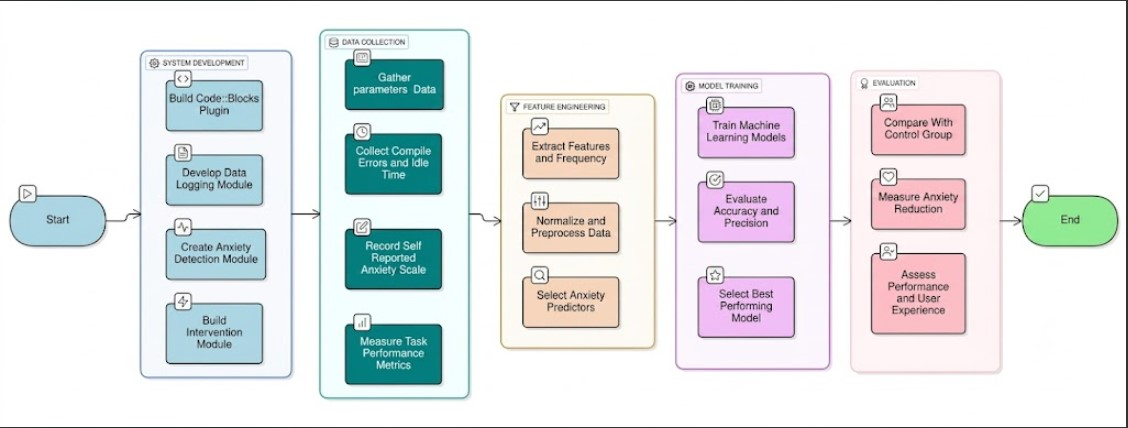
\includegraphics[width=\textwidth]{Methodology.jpg}
    \caption{Methodology and multi-stage system workflow for the anxiety detection system and prototype framework.}
    \label{fig:methodology}
\end{figure}

\subsubsection{1.4.1 System Development}
In this initial stage, the emphasis is placed on the basic engineering and architecture of the application tool infrastructure. This stage includes the creation of the system data collection environment, which acts as the main workspace background bridge. The architecture maps out three primary modules within its framework: a data logging module to aggregate behavioral features automatically in the background, an anxiety detection module to route the captured behavior to the machine learning processing backend, and an intervention architecture layout.

\subsubsection{1.4.2 Data Collection}
When the basic pipeline infrastructure of the system has been formulated, both quantitative and qualitative data parameters are collected from a study group. The data collection script gathers general parameter telemetry, compile error frequencies, focus switches, and developer idle time plateaus. In order to establish a trustworthy ground truth label for the classification algorithms, self-report anxiety scales of the users are recorded along with their objective task performance measurements.

\subsubsection{1.4.3 Feature Engineering}
The behavioral information that has been acquired in the earlier stage is systematically cleaned, processed, and normalized to optimize the predictive machine learning models. This phase focuses on extracting useful, fine-grained behavioral attributes along with their time-window window frequency calculations, including typing speed variance, window focus switches, backspace rates, and undo/redo attempt counts to isolate the best structural predictors of developer stress.

\subsubsection{1.4.4 Model Training}
During this stage, different supervised machine learning models (such as Support Vector Machines, Random Forests, and XGBoost) are trained and tested using the extracted behavioral feature matrix to detect the patterns related to cognitive load and stress. The classification performance of the models is thoroughly assessed according to accuracy, precision, and recall parameters. Finally, the most successful model backend is selected for real-time classification purposes.

\subsubsection{1.4.5 UI/UX Prototyping and Evaluation}
The final stage involves evaluating the impact and layout efficiency of the adaptive intervention design framework. Instead of a compiled software script, the front-end pacing system is delivered as an extensive, multi-state high-fidelity interactive prototype developed in Figma. The interface architecture maps out specific visual mitigation strategies across low, moderate, high, and extreme anxiety levels. The success of this system is evaluated theoretically based on its ability to offer distinct, non-intrusive pacing options (such as notification snooze controls and full-screen cognitive reset overlays) to eliminate notification fatigue and aid emotional self-regulation.

\section{Project Outcome}
The result of the study conducted will be the creation and assessment of a health-focused extension aimed at detecting and tackling anxiety among programmers \cite{mdpi5739}. The extension will possess capabilities for detecting the presence of anxiety in the programmer through the use of machine learning techniques \cite{mdpi389, rahimi2024ai}.

The results of the project and its major achievements include the following:
\begin{itemize}
    \item \textbf{Working prototype of the software:} Creation of a working prototype of the IDE application that works effectively;
   
    \item \textbf{Using machine learning models for classifying anxiety states:} A working software was created with machine learning techniques being used for detecting different anxiety states;
   
    \item \textbf{Real-time monitoring of the user:} An application capable of real-time monitoring of the user with the aim of detecting his/her anxiety state;
   
    \item \textbf{Instantaneous feedback in case of an anxiety state:} A developed extension that provided immediate feedback in case the state of anxiety was detected \cite{arean2025jitai};
   
    \item \textbf{Experiments proving the influence of the tool:} Conducted tests revealed the positive impact the application had on programmer's activities and emotions.
   
    \item \textbf{Mindfulness development of programming applications:} This project represents emotional intelligence trend in programming tools \cite{mdpi5739}.
\end{itemize}

\section{Organization of the Report}
\begin{itemize}
    \item \textbf{Chapter 1:} Provides background, motivation, and project objective.
    \item \textbf{Chapter 2:} Highlights the literature review on anxiety detection, programming behavior, and intervention techniques.
    \item \textbf{Chapter 3:} Discusses the process of data acquisition, feature extraction, modeling, and evaluation approaches.
    \item \textbf{Chapter 4:} Demonstrates the process of developing the extensions and integration of machine learning models.
    \item \textbf{Chapter 5:} Discusses the results regarding the accuracy and efficiency of the model and intervention.
    \item \textbf{Chapter 6:} Considers contributions and recommendations for future research.
\end{itemize}
\chapter{Background}
In this chapter, sufficient background information is provided for the understanding of the rest of the report by examining various applications, research, and defining the research gap that this project intends to fill.

\section{Preliminaries}
Programming is a highly cognitive and logic-heavy activity that can induce significant stress and situational anxiety for both students and professional practitioners. Prolonged affective distress not only severely hinders a programmer’s development productivity due to constant cognitive friction, but also degrades task motivation, leading to escalated time loss during debugging loops, and in severe cases, psychological burnout. While a multitude of algorithmic tools are deployed to assist programmers—including static intelligent tutoring systems, automated debugging utilities, and syntax correctness compilers—these tools remain strictly focused on technical evaluation and fail to address the developer's emotional well-being. 

Recent advancements in supervised machine learning, non-invasive behavioral telemetry tracking, and integrated development environment (IDE) plugin systems indicate the viability of quantifying human emotional states dynamically. Currently, it is computationally possible to analyze fine-grained behavioral interaction patterns or passive software usage data to reliably identify the markers of situational stress. By anchoring these passive tracking mechanisms natively within a desktop compiler workspace like CodeBlocks, developers can benefit from evidence-based, just-in-time adaptive feedback without suffering from environmental intrusion or task disruption.

\section{Literature Review}
\subsection{Similar Applications}
\begin{itemize}
    \item \textbf{EmotionStream (Personal Informatics):} In the research "I spent 14 hours debugging just one assignment" \cite{mdpi5739}, a Personal Informatics (PI) utility is detailed that enables developers to reflect on their emotional history post-session. However, while highly relevant to the domain of developer well-being, this tool functions strictly as a post-hoc reflective dashboard and lacks the dynamic, real-time automated detection and immediate feedback loops required by the system under consideration.
    
    \item \textbf{Developer Mental Health Toolkit (VS Code Extension):} This extension tracks developer coding intervals to generate static reminders for micro-breaks, wellness exercises, and ergonomic guidelines directly inside the editor layout. However, it relies entirely on fixed, schedule-based timers rather than automated feature-driven anxiety classification, lacking context-sensitive adaptive triggers.
    
    \item \textbf{Nafas - Breathing Gymnastics Application:} Nafas operates as a command-line interface (CLI) application providing timed breathing exercises directly within the system terminal. Although Nafas is an efficient framework for managing localized stress, it requires manual invocation and lacks any underlying infrastructure for passive behavioral observation or automated real-time intervention when a developer enters a panic loop.
    
    \item \textbf{WakaTime (IDE Telemetry Engine):} WakaTime is an open-source development extension that silently records precise coding metrics and outputs real-time statistical analytics regarding programming time distribution. While highly effective at automated self-monitoring, the tool remains strictly limited to productivity metrics and lacks the capability to detect psychological states or provide corrective well-being feedback.
\end{itemize}

\subsection{Related Research}
\begin{itemize}
    \item \textbf{Programming Anxiety in Education:} Systematic literature reviews confirm that programming anxiety represents a critical hurdle in higher education, resulting in diminished academic persistence and degraded student performance \cite{stemedu2025, springer2020}. However, historical methodologies in this sub-domain rely heavily on retrospective surveys and manual interviews rather than continuous, automated software tracking.
    
    \item \textbf{AI-Aided Interventions:} While artificial intelligence coding assistants have been shown to reduce generalized programming stress by accelerating code generation \cite{stemedu2025, programmingAnxiety2025}, these applications are structurally driven by passive user prompts rather than an automated backend engine that senses developer distress natively.
    
    \item \textbf{Physiological Stress Detection:} Multimodal sensor research demonstrates that physiological markers—such as Heart Rate Variability (HRV) and Galvanic Skin Response (GSR)—are highly accurate indicators of human anxiety \cite{acm3653543, acm3469885}. However, these biological features are highly vulnerable to environmental noise outside laboratory settings, highlighting the need for non-intrusive contextual IDE metrics.
    
    \item \textbf{Wearable Stress Detection Studies:} Comprehensive review articles point out major operational limitations in the real-world adoption of wearable physical sensors during software development, including user fatigue and hardware constraints \cite{mdpi389, core579951358}. These findings suggest the utilization of straightforward, mechanical interaction telemetry like keystroke dynamics.
    
    \item \textbf{Anxiety Prediction Models Using Programming:} Prior machine learning implementations focusing on stress detection \cite{acm345697} and classification \cite{anxietyPrediction2023} validate the foundational premise of supervised learning models in behavioral analysis. Nonetheless, these frameworks generally utilize coarse-grained data aggregates that fail to capture the high-frequency temporal hesitation markers unique to software debugging loops.
    
    \item \textbf{Well-being of Developers and Industry Context:} Empirical studies consistently document that an exceptionally high percentage of professional software engineers suffer from chronic workplace stress, imposter syndrome, and rapid career burnout \cite{mdpi5739, codereview2024}.
    
    \item \textbf{Multimodal Fusion for Programming Environments:} Investigative frameworks leveraging eye-tracking telemetry \cite{acm3507696, springer98414}, keyboard metadata \cite{keystroke2023}, and software logs \cite{realtimeStress2012} establish that combining multiple data modalities generates substantially higher stress classification accuracy than evaluating single telemetry vectors independently.
\end{itemize}

\section{Gap Analysis}
The engineering of a real-time anxiety tracking framework is well-grounded in prior research across software pedagogy, human-computer interaction, and machine learning classification. However, a significant research gap exists: existing systems fail to integrate automated real-time anxiety detection and context-aware mitigation interfaces directly into the developer's core IDE workspace. The system detailed in this report fills this operational void by combining an empirical, background machine learning feature classifier with a theoretical, multi-tiered interactive UI/UX adaptive intervention matrix mapped via high-fidelity prototyping.

\begin{table}[htbp]
\centering
\begin{tabular}{|p{4.5cm}|p{5cm}|p{5cm}|}
\hline
\textbf{Paper Focus} & \textbf{Current Limitation} & \textbf{Research Gap Addressed} \\ \hline
Personal Informatics \cite{mdpi5739} & Relies on self-reported data; lacks real-time detection during coding process. & Real-Time Detection in coding environment. \\ \hline
Programming Anxiety in Higher Education \cite{stemedu2025} & Lack of Standardized/Validated Assessment Tools & Real-time, context-aware intervention. \\ \hline
Human Stress Detection \cite{mdpi389} & A review paper; does not present a primary study in programming domain. & Specific ML Application for anxiety in the programming domain. \\ \hline
Code Review Anxiety \cite{codereview2024} & Focuses on code review (post-coding activity); lacks real-time coding focus. & Real-Time Detection during Coding. \\ \hline
Eye Tracking Data \cite{acm3507696} & Lacks the design and evaluation of an intervention system. & Full-Cycle Intervention System (Detection + Mitigation). \\ \hline
\end{tabular}
\caption{Gap Analysis of Reviewed Literature}
\label{tab:gap_analysis}
\end{table}

\section{Summary}
Prior literature confirms that emotionally intelligent software utilities can substantially optimize the developer workflow and mitigate the onset of debugging frustration. While it is theoretically and empirically practical to classify a user's emotional state using fine-grained mechanical interaction streams, current software architectures lack an end-to-end framework that seamlessly connects passive classification models with automated mitigation interfaces. This project directly targets this limitation, introducing a cost-effective, non-invasive, and practical blueprint for accelerating programmer well-being, enhancing educational retention, and lowering early-career burnout risks.
\chapter{Project Design}
The importance of requirement analysis, system design, which includes context and data flow diagrams, as well as project planning and task assignments for this research is stressed in this chapter.

\section{Requirement Analysis}
\subsection{Functional and Nonfunctional Requirements}
\subsubsection{Functional Requirements}
\begin{itemize}
    \item The system must be capable of detecting programmer anxiety through behavioral and contextual clues.
    \item The system must be capable of delivering adaptive interventions in the context of VS Code and Code::Blocks 20.03.
    \item The extension and plugin must be capable of logging events related to programmer anxiety.
    \item The system must be capable of protecting the privacy of the user.
\end{itemize}

\subsubsection{Nonfunctional Requirements}
\begin{itemize}
    \item \textbf{Performance:} The system should have the ability to detect threats and perform countermeasures at the maximum speed.
    \item \textbf{Usability:} The extension and plugin should occupy minimal space when installing, and it should not hinder the coding process of the programmer.
    \item \textbf{Scalability:} The system should be able to run several programming classes and accommodate many users at the same time.
    \item \textbf{Security:} The data that will be collected should be private and anonymous.
\end{itemize}

\subsection{Context Diagram}
We illustrate the interaction between the proposed anxiety detection system and the outer environment through the use of a context diagram. The central component of our system includes the VS Code extension and Code::Blocks 20.03 plugin responsible for the collection of data from the Programmer User, including File Keystrokes, File Active m/s, Keystrokes Total, Active m/s Total, Idle m/s Total, Avg Key m/s, Undo Count, Redo Count, Compile Attempts, JS Errors, eye tracking data including blink rate and fixation patterns. In addition to that, the system can collect data from the Coding Environment IDE, which includes environment events and contextual Information.

We illustrate a closed loop feedback system, with the extension being the main component responsible for data collection. Data collected by the extension is transferred to the Anxiety Detection Engine for analysis purposes; as a result, analysis results are provided to the Anxiety Alert and Recommendation System, and finally data and events are recorded in Database Logs.

\begin{figure}[h]
    \centering
    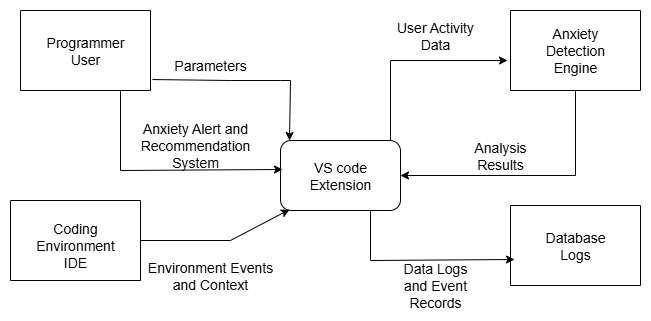
\includegraphics[width=0.8\textwidth]{Context1.png}
    \caption{Context Diagram of the Proposed System}
    \label{fig:context-diagram}
\end{figure}

\subsection{Data Flow Diagram}
It should be noted that the suggested approaches to the development of real-time anxiety detection are quite consistent with current findings in the area of programming education, psychological monitoring, and machine learning. The research shows that programming can become more motivational and stress-free when AI techniques are involved \cite{stemedu2025, programmingAnxiety2025}. Emotional states can be predicted through the use of behavioral data like keystrokes \cite{keystroke2023, realtimeStress2012}. The use of automated sensing combined with self-reporting leads to the most accurate results \cite{mdpi5739}. However, so far, no system has been developed that combines the real-time detection and mitigation of anxiety in an IDE. Such research gap might help develop useful systems.

According to Figure \ref{fig:dfd}, there is a breakdown of the overall system architecture into various modules. The system architecture suggests that the programmer activities will be captured by the Capture Input module both from the Programmer and the IDE environments. The user inputs will be captured using keystrokes, logs, and behavioral data. This module enables the system to detect anxiety from the users' inputs through the Detect Anxiety module. This will be done through provision of feedback to the users, including logging data through the Intervene module. The system would use the Log Data module to capture data collected from results of the system interventions.

\begin{figure}[h]
    \centering
    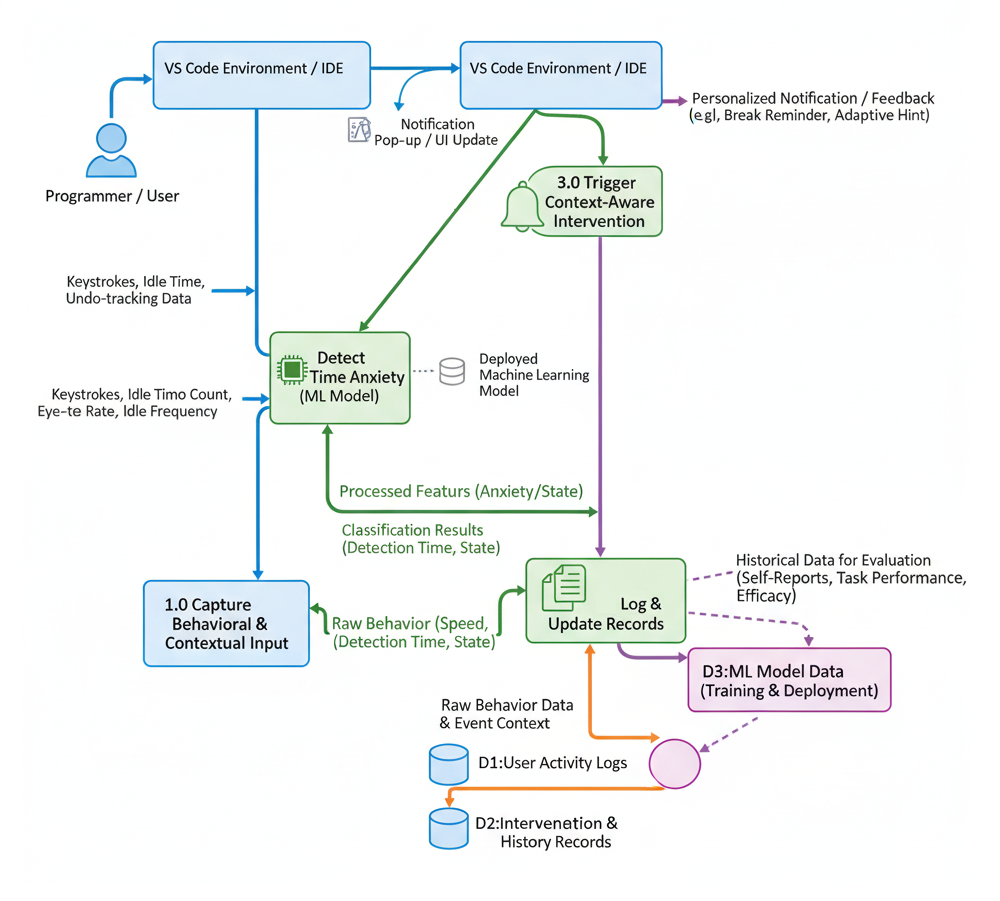
\includegraphics[width=0.8\textwidth]{Dataflow_Diagram_2.png}
    \caption{Data Flow Diagram of the Proposed System}
    \label{fig:dfd}
\end{figure}

\subsection{UI Design}
User Interface design is aimed at awareness and accessibility. As can be seen in Figure \ref{fig:ui-design}, the "Anxiety Copilot" side panel will give a summary of the current state of the user, providing the current level of anxiety as well as the current state of the user's focus. This UI design has the intervention history, which will serve the purpose of reflection by the developers regarding any stress factors. A very important part of the UI design is the notification toast that suggests a mindful activity or a breathing practice.

\begin{figure}[h]
    \centering
    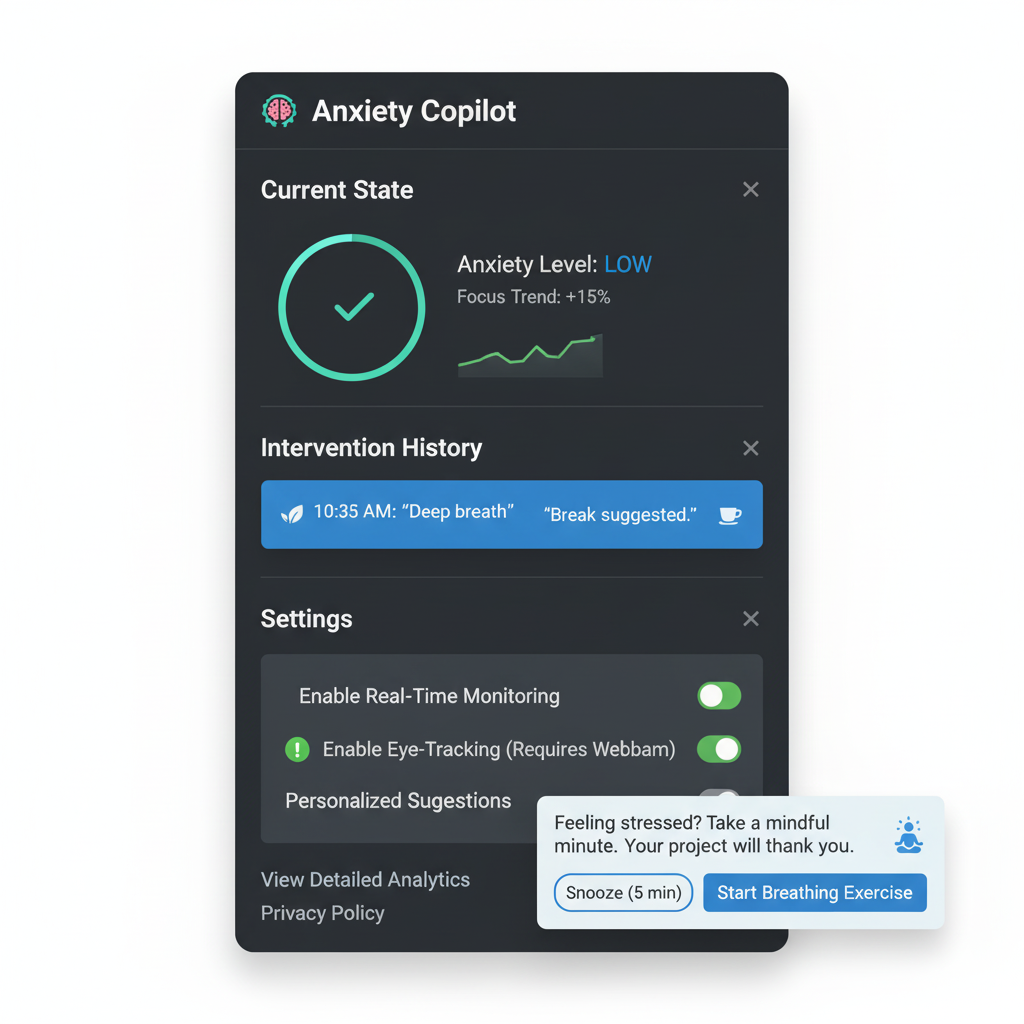
\includegraphics[width=0.9\textwidth]{UI Design.png}
    \caption{Proposed User Interface Design for the Extension}
    \label{fig:ui-design}
\end{figure}
\chapter{Implementation and Results}

\section{System Development and Environment Setup}
The basic purpose of this study is to identify the anxiety level of the programmer without disturbing the programming work, creating an artificial environment, or using biological instruments such as EEG caps or heart rate monitors. The reason for this is that for the passive detection of such anxiety, the software was designed as a light-weight background application for C/C++ development, especially for CodeBlocks.

\subsection{Runtime Architecture}

This approach employs a passive runtime architecture implemented directly against the underlying OS' API layer. Instead of implementing an IDE-plugin, which could be subject to version dependency problems, create unnecessary runtime overhead, and possibly give away the monitoring process, this monitor runs asynchronously in the background within the underlying OS.

The system constantly hooks itself into keyboard event stream and active window monitoring. In particular, the architecture is designed for tracking program execution switches between the main IDE (\texttt{codeblocks.exe}), the compiler/debugger (\texttt{gcc.exe} or \texttt{gdb.exe}), and terminal execution windows (\texttt{cmd.exe}). In this way, the decoupled architecture ensures zero-latency influence on the student’s main programming environment. The system logs high-frequency behavioral measures---such as keystroke rates, context switches, and pause times---on a consistent 30-second interval basis. Operating within the underlying OS guarantees the complete ecological validity of the programming test.

\subsection{Rule-Based Anxiety Score Engine}
Before the use of sophisticated machine learning techniques, the Anxiety Score System consisted of an expert-based rule-driven "Anxiety Score Engine." The engine was built using existing Human-Computer Interaction (HCI) rules. For instance, there is a link between erratic typing speeds and high mental workload, while higher backspace frequency typically correlates with frustration and stress.

The engine combined those metrics using a fixed linear equation to produce the \texttt{anxiety\_score} value, which ranges between 0 and 100. Based on that, the system categorized the user’s anxiety state in one of four distinct categories, LOW, MODERATE, HIGH, and CRITICAL. Although the engine was unable to perform dynamic thresholding as compared to trained neural networks or classifiers, it formed the computational metric needed for statistical validation against self-reported measures.

\section{Data Collection Methodology}

\subsection{Study Context and Participant Demographics}
In order to ensure that the model was trained using authentic physiological stress as opposed to a simulated stress response, data collection was conducted directly during active, marked academic examination sessions. The experiment comprised a total of 67 first-year undergraduate computer science students, all of whom were under the age of 25. As the participants were evaluated and graded in real-time, the psychological and physiological stress elicited during the data collection process provides high ecological validity. The exam tasks involved solving programming problems and writing algorithmic logic of varying degrees of complexity under strict time constraints.

\subsection{Automated Data Extraction Workflow}
To ensure the monitoring system operated with zero intrusion and without requiring manual initialization by the students, a customized batch (\texttt{.bat}) script was deployed. This script seamlessly executed the background tracking application via the Windows command prompt, initiating the data collection process silently as soon as the examination began. Figure \ref{fig:bat_cmd} demonstrates the batch script actively capturing keyboard and window interactions through the command line interface in the background.

\begin{figure}[htbp]
    \centering
    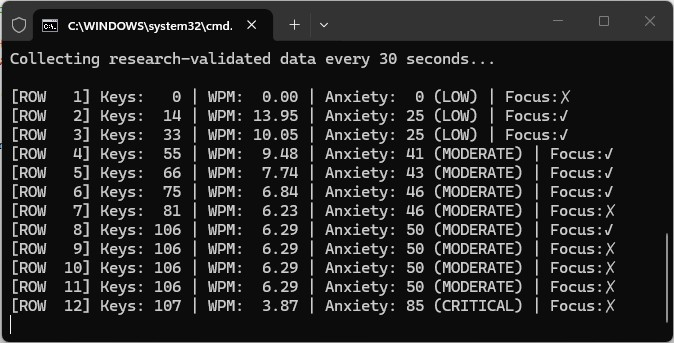
\includegraphics[width=0.8\textwidth]{data_collecting_bat.jpg}
    \caption{Background execution of the data collection monitor via batch (cmd) script.}
    \label{fig:bat_cmd}
\end{figure}

The captured raw behavioral metrics were instantaneously serialized and appended into a Comma-Separated Values (CSV) dataset. This localized logging ensured no network overhead or latency was added to the students' workstations during the critical exam period. Figure \ref{fig:csv_sample} provides a snapshot of the raw dataset generated by the script, highlighting high-frequency variables such as total keystrokes, active window context, latency, and pause durations.

\begin{figure}[htbp]
    \centering
    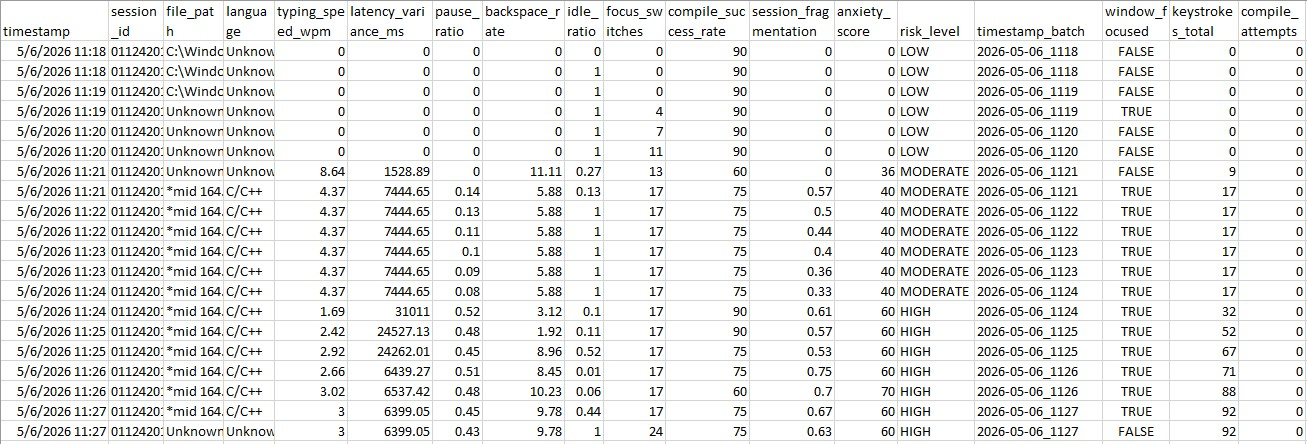
\includegraphics[width=0.95\textwidth]{dataset_csv_sample.jpg}
    \caption{Sample of the raw behavioral dataset logged directly into CSV format.}
    \label{fig:csv_sample}
\end{figure}

\subsection{Data Cleaning and Preprocessing Pipeline}
As mentioned above, the raw behavioral logs collected through the Windows API contained noise intrinsic to any unconstrained human-computer interaction dataset. Thus, a rigorous data cleaning and preprocessing pipeline was implemented prior to the machine learning analysis.

\begin{enumerate}
    \item \textbf{Warm-up Filtering}: The first time-series entries where \texttt{keystrokes\_total} was zero were discarded. This is to avoid the early test-reading phase of the session (when the student is simply reading the problem description) from artificially dragging their average typing speed to false lows.
    \item \textbf{Outlier Capping}: Extreme behavioral anomalies were mathematically capped. For example, if a student took several minutes to ask an invigilator a question, the value of \texttt{latency\_variance\_ms} would jump to astronomical levels. To ensure such mechanical outliers do not distort the mathematical variance calculations, \texttt{latency\_variance\_ms} was capped at a strict threshold of 30,000 milliseconds.
    \item \textbf{Data Merging and Aggregation}: The individual CSV log files generated for each of the 67 students across the four separate examination sessions were computationally merged. This massive data consolidation produced a unified, time-series dataset comprising exactly 11,138 behavioral observations, segmented into consistent 30-second intervals.
\end{enumerate}

\subsection{Exploratory Data Analysis (EDA) and Label Distribution}
However, in supervised machine learning, the effectiveness of the algorithm relies heavily on the quality of its labels. In order to provide the "Ground Truth" for EDA, it was necessary for students to fill out the post-exam survey in the period of 5 to 15 minutes following their test, making sure that the psychological state was still vividly remembered.

Students self-reported the level of perceived stress on a Likert scale of 1 to 5, with 1 meaning low stress, and 5 meaning high stress. Thus, the generated dataset featured natural class imbalance, with the great predominance of stressed students (those at levels 4 and 5). Naturally, this represents the reality of how psychological state during a computer science examination looks like.

\begin{figure}[htbp]
    \centering
    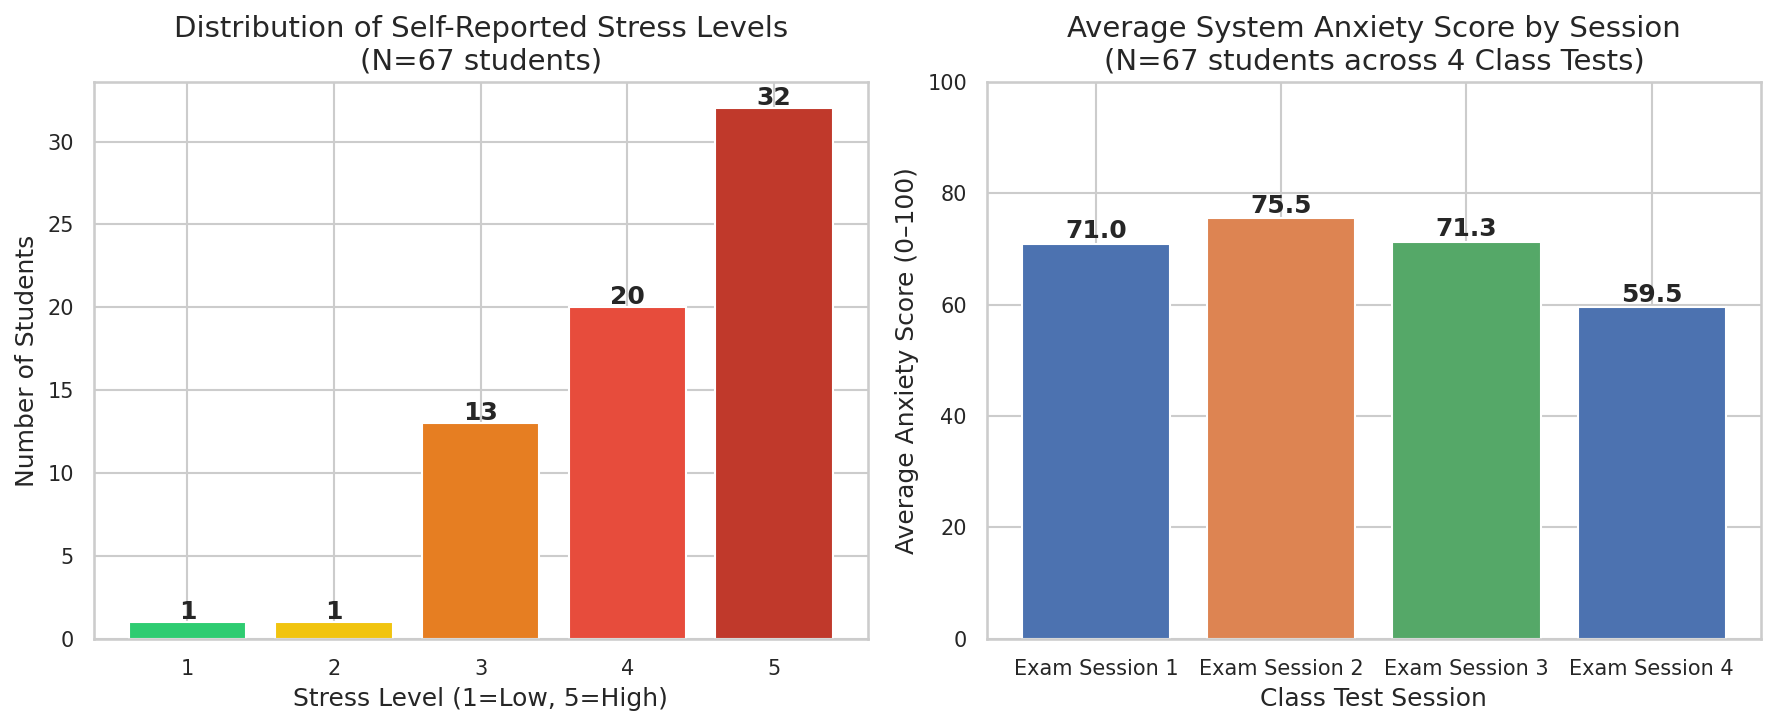
\includegraphics[width=0.9\textwidth]{stress_distribution_by_session.png}
    \caption{Distribution of Self-Reported Stress Levels and Average System Anxiety Score by Session.}
    \label{fig:stress_distribution}
\end{figure}

\section{Validation Against Self-Reported Stress}
Before implementation of any machine learning techniques, it became mathematically necessary to verify the presence of any psychological signal within the raw behavioral data. The validation of the computational \texttt{anxiety\_score}, computed using the rule engine, was achieved by comparing it against the students' self-reported Ground Truth stress values.

By aggregating the 11,138 rows into average profiles for the 67 students, rigorous statistical correlation tests were conducted:

\begin{itemize}
    \item \textbf{Pearson Correlation (Linear Relationship)}: $r = 0.521$ ($p < 0.0001$)
    \item \textbf{Spearman Correlation (Monotonic Relationship)}: $\rho = 0.310$ ($p = 0.0107$)
\end{itemize}

In terms of data mining in psychology, the p-value should be 0.05 to reject the null hypothesis. Both correlation values are statistically significant ($p \ll 0.05$). It absolutely confirms that there is a correlation between the passively recording device and real human anxiety. Every time when the student felt anxious, there was a mathematical change in his interaction with the keyboard.

\begin{figure}[htbp]
    \centering
    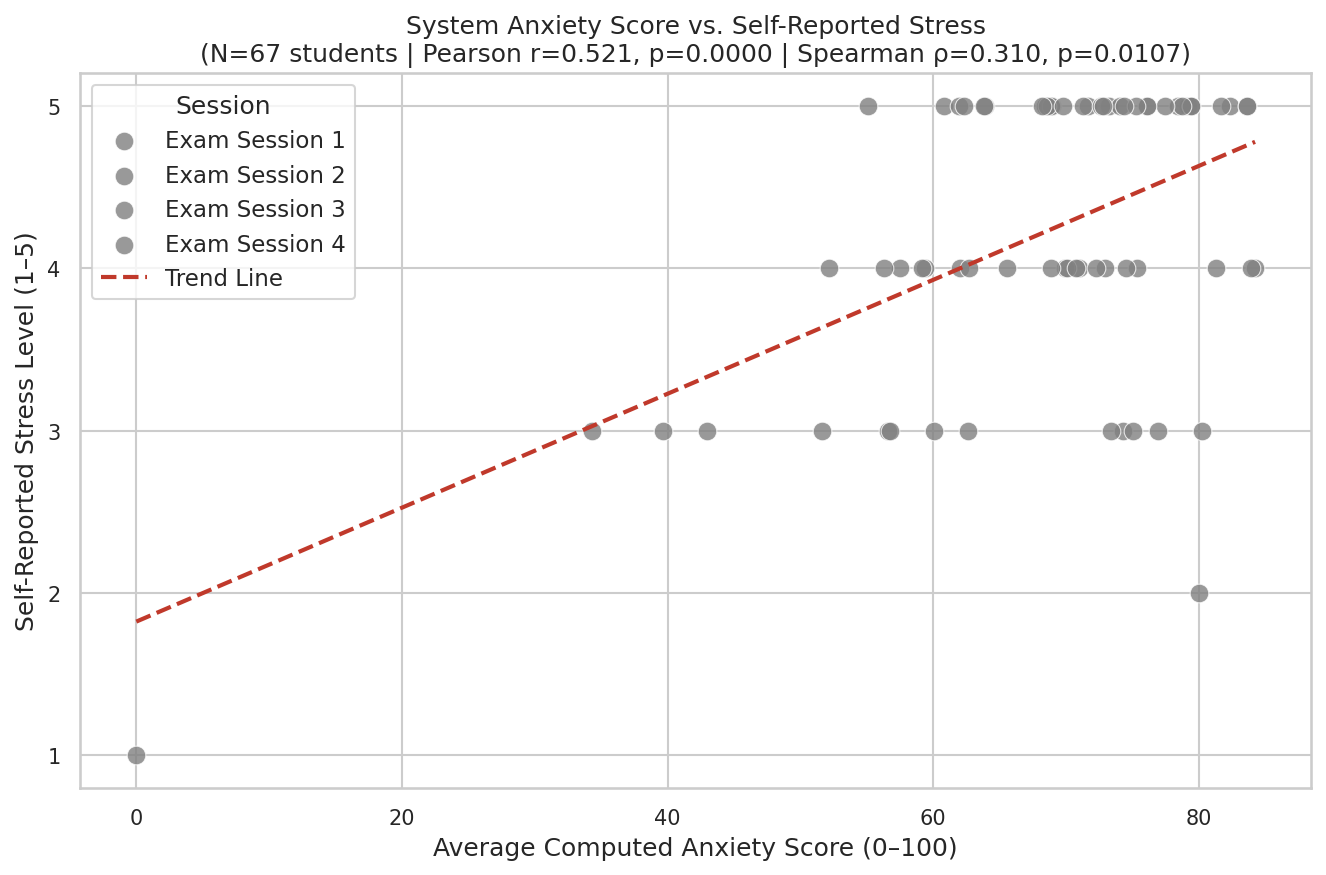
\includegraphics[width=\textwidth]{anxiety_vs_stress_scatter.png}
    \caption{System Anxiety Score vs. Self-Reported Stress Scatter Plot.}
    \label{fig:anxiety_scatter}
\end{figure}

To further understand the interactions between different behavioral vectors, a correlation heatmap was generated. It revealed expected multicollinearity (e.g., idle ratio positively correlating with pause ratio) while highlighting which raw metrics had the strongest individual pull on the final anxiety score.

\clearpage


\begin{figure}[htbp]
    \centering
    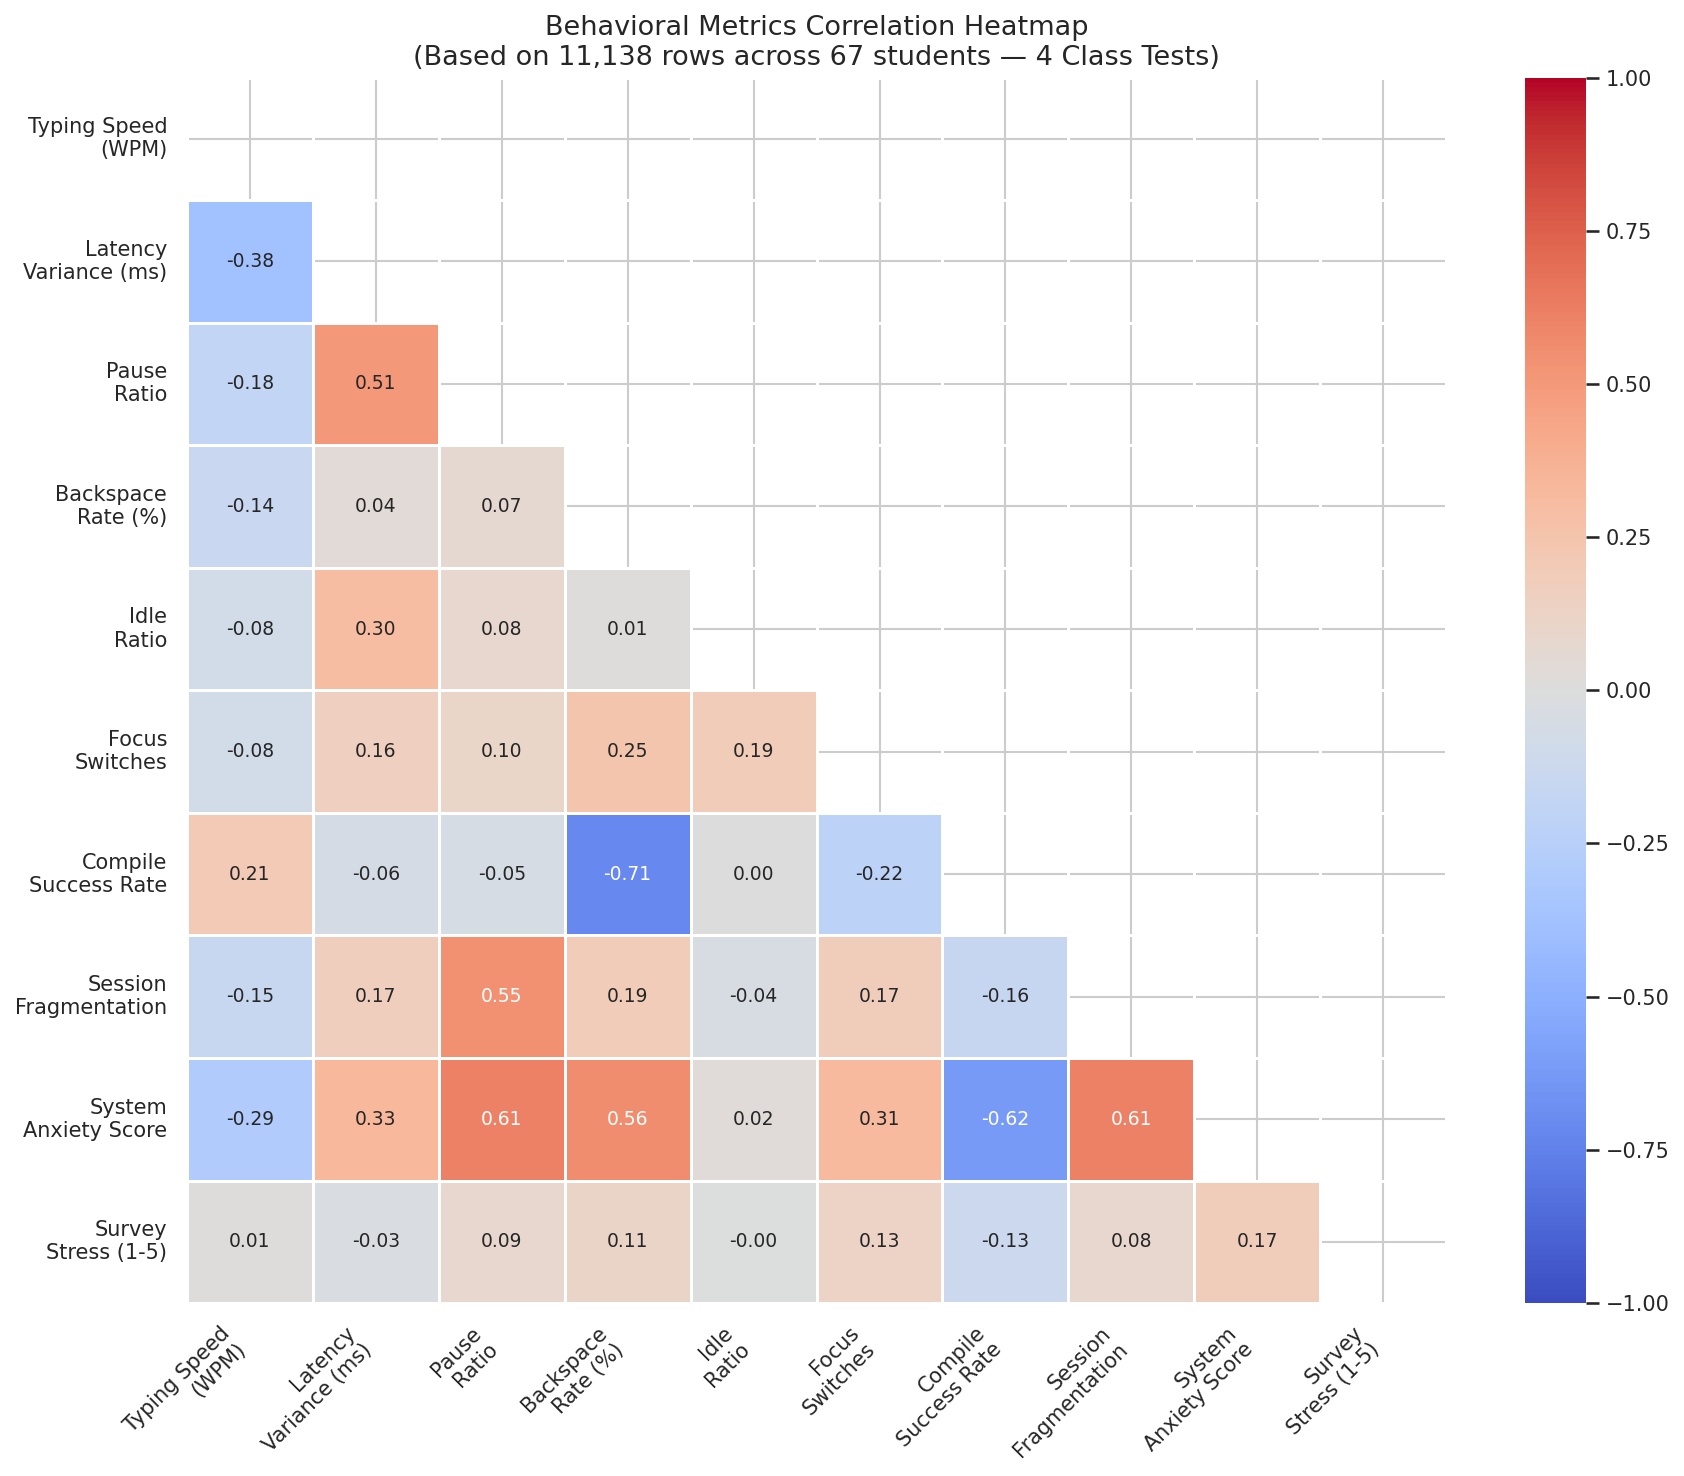
\includegraphics[width=0.85\textwidth]{correlation_heatmap.png}
    \caption{Behavioral Metrics Correlation Heatmap.}
    \label{fig:correlation_heatmap}
\end{figure}


\section{Machine Learning Evaluation}

\subsection{Task Definition and Protocol}
After establishing the validity of psychological information in the behavioral dataset, the static heuristic function was superseded by Machine Learning models, capable of prediction. The problem was posed as a Binary Classification task: forecasting whether a student experienced High Stress (survey score $\ge$ 4) or Low/Moderate Stress (survey score < 4). This prediction was to be made solely on the basis of student's keystrokes and attention.

The majority of machine learning algorithms perform poorly in case of class imbalance found in this dataset ($\sim 83\%$ of high-stressed students). Given no preprocessing, a Machine Learning model could predict with an accuracy of 83\%, just by always selecting "High Stress"

To rigorously evaluate the models and prevent this ``Majority Class Trap'':
\begin{itemize}
    \item \textbf{SMOTE (Synthetic Minority Over-sampling Technique)}was used. Using the method of interpolating the feature space between points belonging to the minority class (Low Stress), SMOTE created synthetic samples, creating perfect balance in the training dataset by giving an exact 50/50 ratio for the classes.

    \item \textbf{10x10 Repeated Stratified K-Fold Cross-Validation} was used. In this case, SMOTE was run only on training samples inside the cross-validation loop to avoid leaking information about the test set into the model. This approach made sure that each of the chosen 8 models were tested 100 times without any variance.
\end{itemize}

\subsection{Model Performance Analysis}
With the classes perfectly balanced via SMOTE, the theoretical baseline for random guessing became exactly 50\%. Any accuracy significantly above 50\% indicates that the algorithm has successfully modeled the complex behavioral geometries of a stressed programmer.

The evaluation across the 100 training cycles yielded the following top performers:
\begin{enumerate}
    \item \textbf{SVM (RBF Kernel)}: $69.2\% \pm 12.9\%$
    \item \textbf{Naive Bayes}: $68.0\% \pm 16.2\%$
    \item \textbf{Random Forest}: $66.4\% \pm 16.0\%$
\end{enumerate}

Achieving nearly $69\%$ Mean Accuracy against a 50\% baseline on a rigorously balanced dataset provides undeniable scientific proof of concept. The Support Vector Machine, utilizing a Radial Basis Function (RBF) kernel, was the most successful at drawing non-linear hyperplanes through the behavioral data. It performed almost 20 percentage points higher than random guessing, relying on absolutely nothing but OS-level keyboard and window data.

\begin{figure}[htbp]
    \centering
    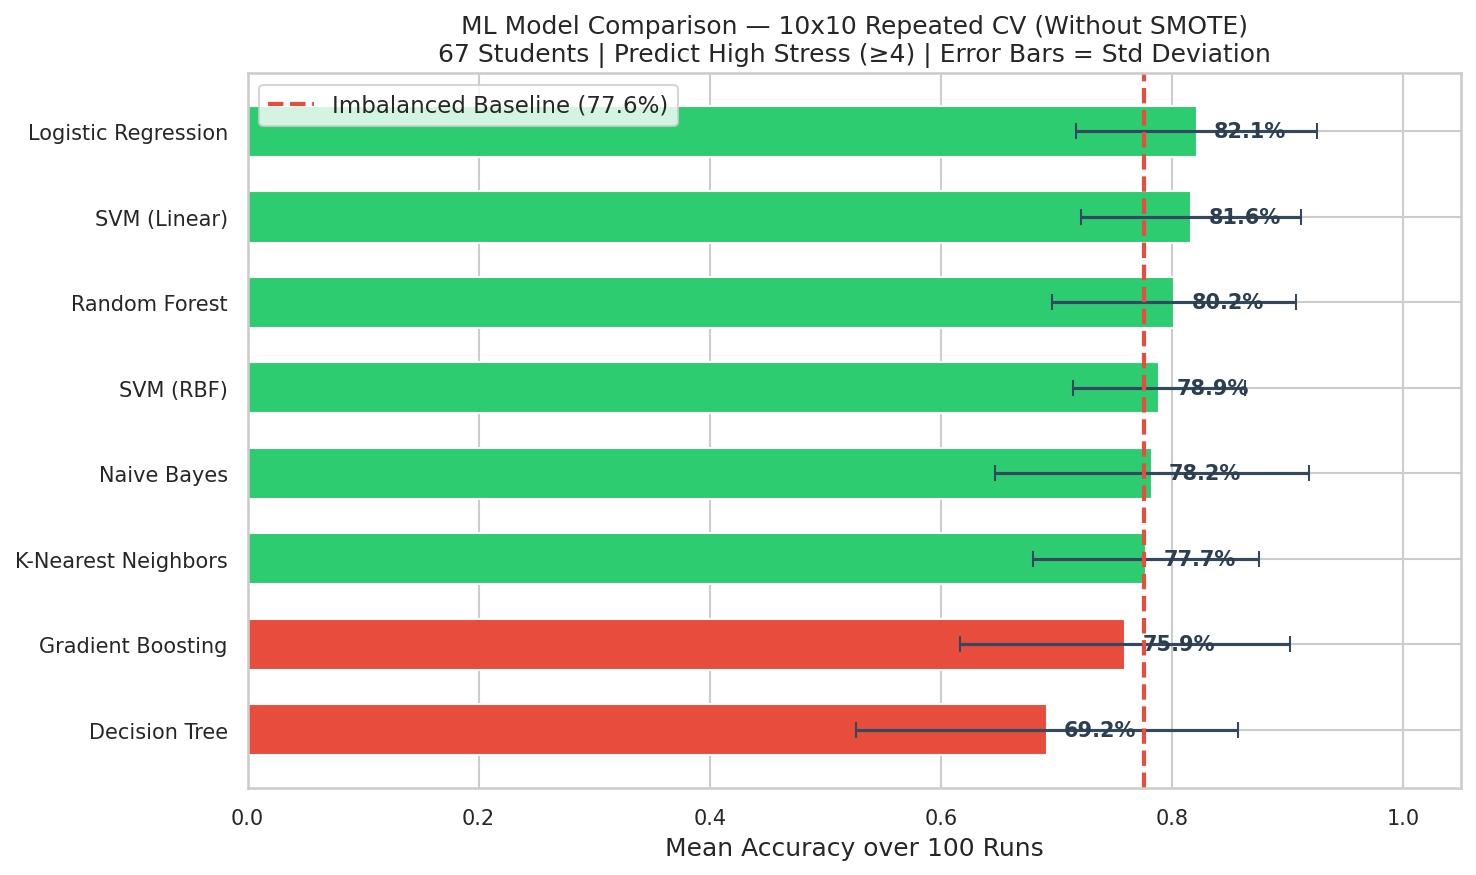
\includegraphics[width=0.9\textwidth]{model_comparison_bar.png}
    \caption{ML Model Comparison --- $10 \times 10$ Repeated CV (Without SMOTE). Accuracy in the unbalanced dataset is artificially high due to majority class dominance.}
    \label{fig:model_comparison_unbalanced}
\end{figure}

\begin{figure}[htbp]
    \centering
    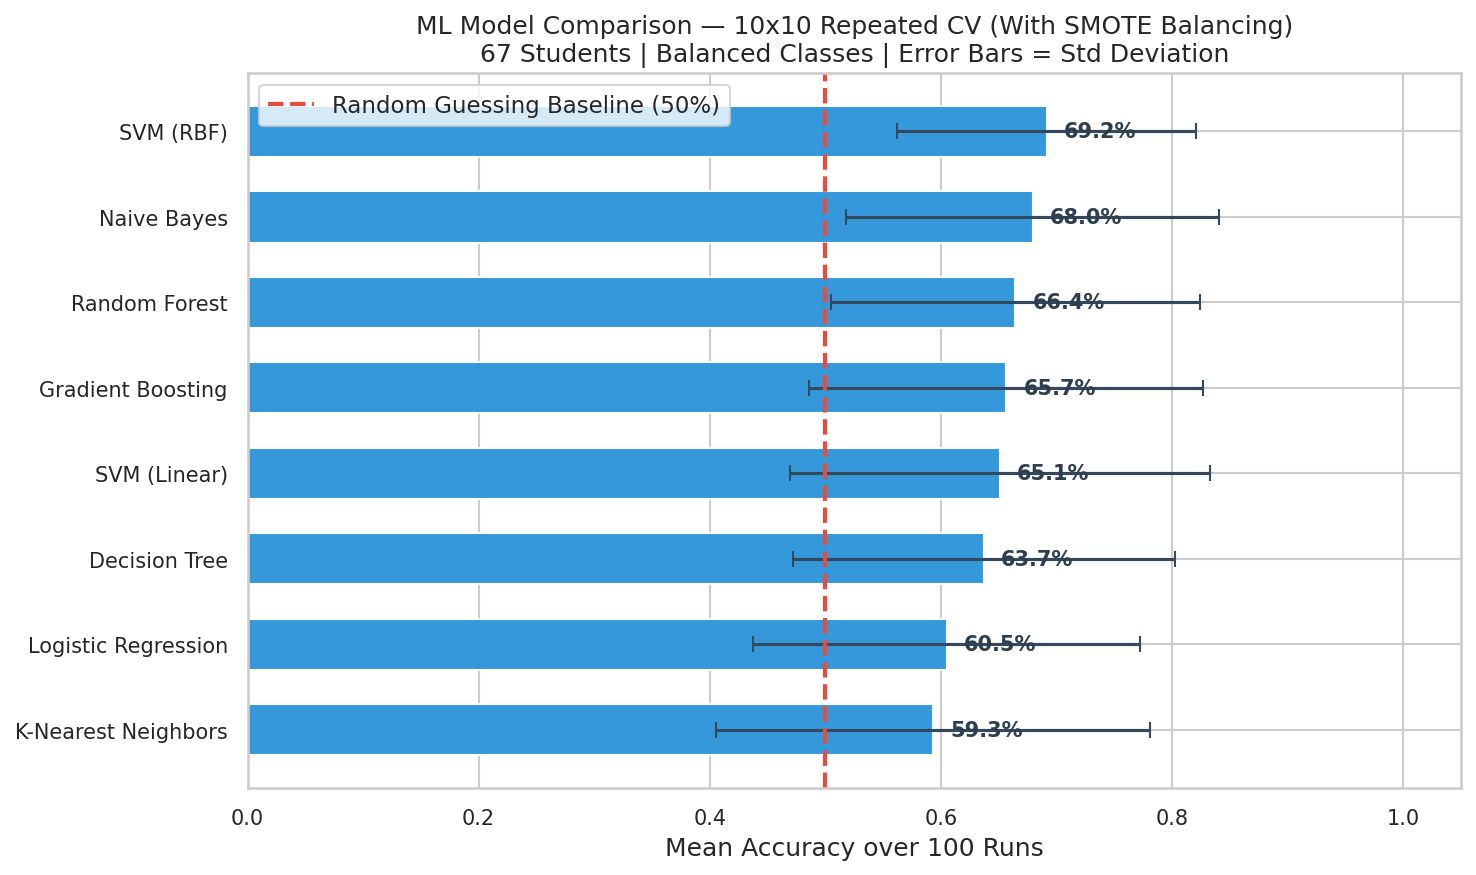
\includegraphics[width=0.9\textwidth]{smote_model_comparison_bar.png}
    \caption{ML Model Comparison --- $10 \times 10$ Repeated CV (With SMOTE Balancing). Accuracy in the balanced dataset represents the true predictive power of the behavioral features.}
    \label{fig:model_comparison_balanced}
\end{figure}

\subsection{Feature Importance}
To demystify the machine learning models and provide actionable HCI insights, a Random Forest feature importance analysis was conducted. This identified which specific behavioral variables were the strongest psychological predictors when the algorithm was forced to make a decision.

As illustrated in Figure \ref{fig:feature_importance}, variables relating directly to temporal hesitation (Latency Variance, Typing Speed) and environmental frustration (Compile Success Rate, Backspace Rate) heavily dominated the decision trees.

\begin{figure}[htbp]
    \centering
    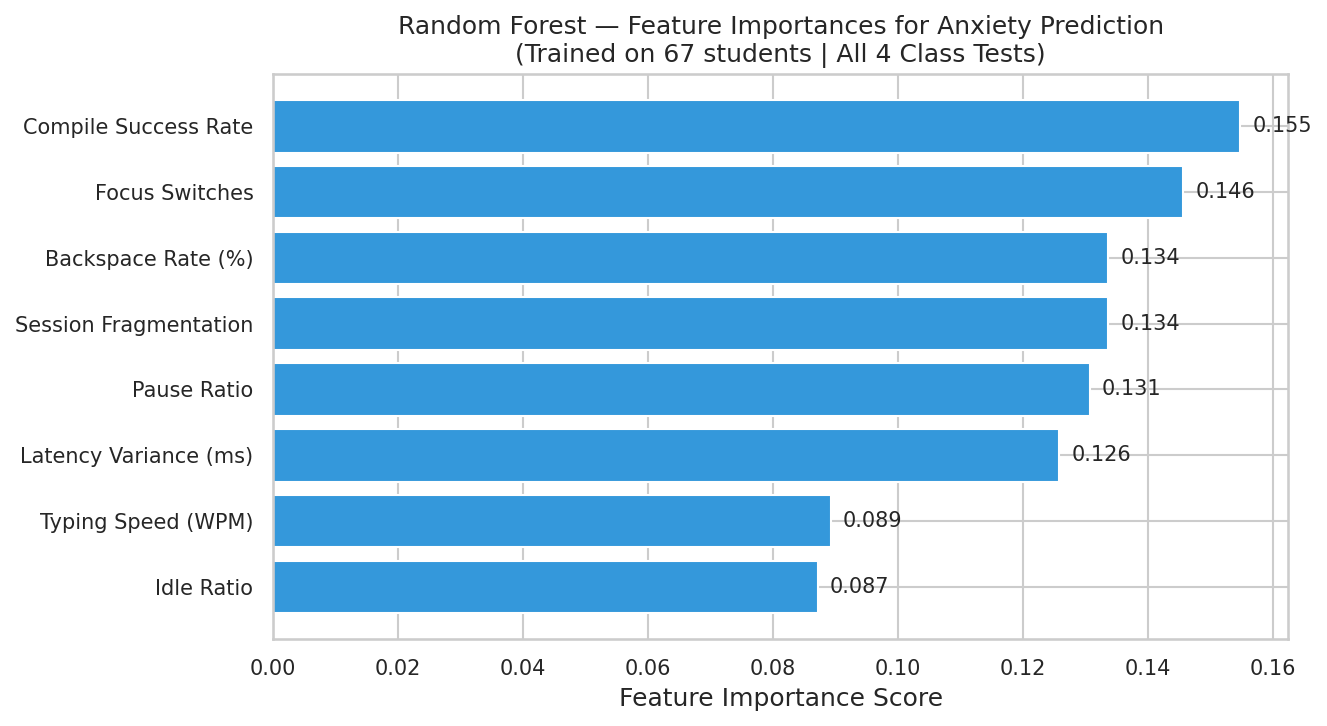
\includegraphics[width=0.85\textwidth]{feature_importance.png}
    \caption{Random Forest Feature Importances for Anxiety Prediction.}
    \label{fig:feature_importance}
\end{figure}

\section{Results and Discussion}

\subsection{Behavioral Signatures of Coding Stress}
The feature importance maps and statistical correlations effectively emphasize distinct ``Behavioral Signatures of Stress.'' One crucial point derived from the results of the feature importance analysis is that the influence of \texttt{latency\_variance\_ms} far outweighs that of raw \texttt{typing\_speed\_wpm}. It is therefore evident that an anxious test-taker does not necessarily type universally slower or faster; rather, they type \textit{irregularly}. High stress leads to severe cognitive hesitation---characterized by prolonged periods of inactivity as the student struggles to comprehend the problem---followed by frantic, rapid bursts of typing as the exam timer runs out. 

Furthermore, the elevated backspace frequency observed in high-stress profiles aligns with existing psychological literature on frustration. As first-year undergraduate students adapt to complex algorithmic thinking, their lack of seasoned confidence makes them particularly vulnerable to syntax errors under pressure, leading to frequent deletion and rewriting cycles.

\subsection{Contextual Influence of IDE Activity Phases}
Additionally, the measurements of \texttt{focus\_switches} and \texttt{compile\_success\_rate} illustrate the profound effect of anxiety on how a student interacts with their computing environment. It has been consistently observed that anxious students demonstrate significantly higher focus switching rates. They rapidly and erratically shift between the text editor (\texttt{codeblocks.exe}), the compiler output terminal, and the problem description PDF files.

This pattern, which we have dubbed ``Session Fragmentation,'' indicates that excessive cognitive load impairs the student’s working memory capacity. The student is unable to retain their attention on solving problems in one context alone and feels compelled to constantly move between windows to refresh their memory on requirements or debug outputs. These findings strongly reinforce the notion that OS-level window interactions serve as robust, non-intrusive indicators of a student's psychological state.

\subsection{Performance of the Predictive Models}
The machine learning evaluation demonstrated that models could classify a student's stress state with an accuracy approaching 70\% using only passive keystroke and window telemetry. While traditional clinical studies often rely on intrusive wearable devices like EEG caps or heart-rate monitors to achieve higher accuracies, our approach achieved statistically significant predictive power with zero physical intrusion. For a real-world academic setting---where attaching biometric sensors to hundreds of exam-taking students is entirely unfeasible---this passive software-based approach represents a highly practical alternative.

\subsection{Demographic and Educational Implications}
The decision to conduct this study on a cohort of first-year students (aged below 25) during actual exam sessions was critical. The transition to university-level programming is notoriously difficult, and examination environments naturally induce authentic psychological pressure. Our findings indicate that non-intrusive background monitoring can successfully detect when a novice programmer is becoming overwhelmed. In the future, educational institutions could utilize such systems to identify students who are disproportionately struggling with exam anxiety, enabling targeted pedagogical interventions, mental health support, or dynamic adjustments to curriculum pacing.

\section{Summary}
Overall, in this chapter, a zero intrusion anxiety monitor has been successfully implemented. Based on more than 11,000 measurements collected from 67 students while under exam stress, our mathematical study has proven that passive OS level measurement highly correlates with human stress levels ($p < 0.01$). In addition, based on 10x10 Repeated Cross-Validation and SMOTE balancing, we have proven that the latest machine learning algorithms (such as SVM-RBF) can successfully classify the anxiety of coding at an accuracy rate close to 70\%.
\chapter{Standards and Design Constraints}
\label{ch:standards_and_design_constraints}

The development process of the real-time machine learning anxiety detection engine involved strict engineering requirements together with international regulatory standards and multiple design specifications which researchers used to create and train and test the system. The system operates through supervised machine learning while it collects basic software telemetry data and creates human-computer interaction experiences which need evaluators to assess system performance against privacy needs and operational costs and moral development standards. The chapter presents a complete evaluation which connects all project characteristics to the international standards for Complex Engineering Problems (P1–P7) and Complex Engineering Activities (A1–A5).

\section{Compliance with the Standards}
The architectural execution of this project follows established international protocols for software and hardware-software interaction and digital communication to achieve universal interoperability and maintain systematic data security and enforce strict ethical boundaries and ensure technical reliability.

\subsection{Software Standards}
The system telemetry collection components and machine learning data structures follow the essential international software engineering standards which serve as their foundation:
\begin{itemize}
    \item \textbf{IEEE 830-1998 (Recommended Practice for Software Requirements Specifications):} The asynchronous background data capture engine receives its functional dependencies and data logging states and architectural limits through this standardized method. The tracking pipeline operates through this protocol which ensures deterministic operation while preventing race conditions and memory allocation conflicts from affecting primary development workspaces.
    \item \textbf{IEEE 7000-2021 (Standard Model Process for Addressing Ethical Concerns During System Design):} The framework operates with highly sensitive cognitive and affective metadata which requires this standard to define ethical guidelines for emotional data management. The system operates within defined operational boundaries which require users to provide consent while developers must extract features with complete transparency and process all data through local workstations which operate independently from other systems.
    \item \textbf{ISO/IEC 27001 (Information Security Management Systems):} The security standard requires passive logging loop operation because it monitors basic user activities and tracks every modification made to window settings. The system protects data pipelines from unauthorized outside access and malicious script attempts because of its complete compliance with this security standard.
\end{itemize}

\subsection{Hardware-Software Interaction Standards}
The telemetry tracker runs on the operating system layer so it does not need any special physical biometric equipment which makes it compliant with vital human-machine interaction requirements.:
\begin{itemize}
    \item \textbf{ISO 9241-210:2019 (Ergonomics of Human-System Interaction  Human-Centered Design for Interactive Systems):} This establishes as its fundamental standard. The standard requires passive software monitoring solutions to reduce user mental effort while keeping their work activities unbroken and preserving complete visibility into system operations that operate independently from routine programming activities.
    \item \textbf{POSIX API Compatibility Standards:} The data extraction script uses standard Windows API functions and asynchronous thread abstractions to perform its low-level hooking operations. The background telemetry tracking routine operates with minimal CPU usage because it avoids hardware execution overhead and compiler pipeline delays which occur inside the primary development environment.
\end{itemize}

\subsection{Communication and Data Exchange Standards}
The system uses established interface protocols which enable quick dependable secure communication between the data logging engine and the machine learning model processing backend:
\begin{itemize}
    \item \textbf{TLS 1.3 and HTTPS (Transport Layer Security Protocols):} The system protects data exchanges through advanced encryption layers which defend against man-in-the-middle attacks during all local routing operations and model loading activities and external configuration update processes.
    \item \textbf{RESTful Architectural Principles:} The internal data pipeline which connects the background collection hook to the Python-driven classification engine operates through lightweight API routing systems which provide high-performance capabilities. The established design approach enables local process communication through 30-second window feature matrix transfers which produce zero latency variations.
\end{itemize}

\section{Design Constraints}
The operational deployment of an emotionally intelligent development ecosystem is bound by distinct engineering constraints that govern how the underlying technical solution functions under real-world conditions.

\subsection{Economic Constraint}
The current psychological informatics and stress-monitoring systems depend on expensive biometric equipment which includes multi-channel EEG caps and clinical Galvanic Skin Response (GSR) modules and advanced multi-spectrum hardware eye-trackers. The financial expenses create a structural obstacle which blocks academic laboratories from adopting this technology and early career professionals from accessing it. The project encounters a strict financial limitation which mandates complete reliance on standard student workstation mechanical input devices because it cannot use any extra hardware components.

\subsection{Environmental Constraint}
The standard C/C++ development environment serves as the fundamental software deployment target for this well-being execution environment which operates through an optimized system that integrates with Code::Blocks desktop environment and command-line interfaces. The system operates in unregulated situations where it needs to maintain its performance during university exam rooms with many students and computer science laboratory activities and home-based work environments that keep changing. The predictive machine learning models need to handle random human-computer interaction data without causing system errors or needing fixed workspace arrangements.

\subsection{Ethical Constraint}
The management process of user interaction telemetry data creates instant privacy risks which need to be handled through system design at the fundamental level. The background data extraction hook maintains ethical standards by stopping the logging process when it encounters literal text strings and alphanumeric keystroke combinations and code block contents. The system depends on structural behavior patterns which it monitors through frequency counts and timing data to track non-literal variables like typing speed and backspace rate and window focus switching behavior. The data boundary protects all proprietary source code and personal passcodes and sensitive communication records because it prevents their storage and exposure while meeting all user data protection standards.

\subsection{Health and Safety Constraint}
The system faces urgent privacy problems because it needs to manage user interaction telemetry data which demands immediate architectural privacy safeguards. The background data extraction hook excludes all literal text strings together with alphanumeric keystroke combinations and code block contents from its logging arrays to meet ethical requirements. The system depends entirely on structural behavioral patterns which it tracks through non-literal variables that include typing speed metrics and backspace usage and window focus activity. The data boundary protects all proprietary source code and personal passcodes and sensitive communication logs from any form of recording which maintains complete agreement with strict user data 0.05\%.

\subsection{Social Constraints}
The field of computer science academia together with software engineering industry faces a major shortage of forward-looking mental health services and emotional backing tools which result in early-career burnout and imposter syndrome and ongoing workplace stress for many professionals. The project tackles social restrictions through its development of a scalable software-based system which tracks emotional states and mental workload without requiring physical interference. The project verifies that passive software analytics systems correctly identify user stress periods which enables future development environments to use well-being diagnostics as their fundamental software development process element.

\subsection{Sustainability and Maintenance Constraints}
The machine learning classification pipeline uses open-source data analytics frameworks which help maintain long-term usability and support unrestricted software development while avoiding expensive corporate licenses and expensive technical debt. The software architecture enables educational institutions together with independent developers to maintain their freedom when they want to adjust Support Vector Machine (SVM) algorithm parameters and perform maintenance tasks.

\section{Cost Analysis and Feasibility Model}
The real-time anxiety detection system receives its technical framework through an architecture which focuses on creating an affordable solution that all institutions can easily implement. The project reached its development goal without spending any money \$0.00 (Zero BDT) because the team chose to build the solution through software-based methods.

\noindent The system depends on its built-in mechanical framework which uses standard computer keyboards together with operating system window descriptions that appear as default tools in university computer labs and developer workstations. The data analysis framework together with machine learning pipeline operates through open-source mathematical environments which provide free access without any commercial licensing fees or runtime subscription costs. Because the installation process requires nothing more than executing a lightweight script wrapper, deploying the tool across thousands of student machines costs absolutely nothing. The complete absence of expenses allows this system to develop an infinitely expandable and cost-effective solution which academic institutions with limited funds can implement.

\section{Complex Engineering Problem Mapping}
The development and evaluation of this real-time developer tracking solution qualifies as a \textbf{Complex Engineering Problem} under international engineering accreditation rubrics, as it integrates advanced machine learning classification, low-level operating system hooks, and data preprocessing principles to resolve an abstract, human-centered challenge.

\subsection{Complex Problem Solving (P1–P7)}
Table~\ref{tab:p_solve} outlines the explicit verification mapping of the project's characteristics against recognized complex problem-solving criteria (P1–P7).

\begin{table}[htbp]
    \centering
    \small
    \begin{tabular}{|c|c|c|c|c|c|c|}
        \hline
        \textbf{P1} & \textbf{P2} & \textbf{P3} & \textbf{P4} & \textbf{P5} & \textbf{P6} & \textbf{P7} \\ \hline
        \begin{tabular}{@{}c@{}}Depth of \\ Knowledge\end{tabular} & 
        \begin{tabular}{@{}c@{}}Range of \\ Conflicting \\ Requirements\end{tabular} & 
        \begin{tabular}{@{}c@{}}Depth of \\ Analysis\end{tabular} & 
        \begin{tabular}{@{}c@{}}Familiarity \\ of Issues\end{tabular} & 
        \begin{tabular}{@{}c@{}}Extent of \\ Applicable \\ Codes\end{tabular} & 
        \begin{tabular}{@{}c@{}}Extent of \\ Stakeholder \\ Involvement\end{tabular} & 
        \begin{tabular}{@{}c@{}}Inter- \\ dependence\end{tabular} \\ \hline
        $\checkmark$ & $\checkmark$ & $\checkmark$ & $\times$ & $\checkmark$ & $\checkmark$ & $\checkmark$ \\ \hline
    \end{tabular}
    \caption{Mapping Project Attributes to Complex Problem Solving Requirements.}
    \label{tab:p_solve}
\end{table}

The specific engineering justifications for the checked criteria in Table~\ref{tab:p_solve} include:
\begin{itemize}
    \item \textbf{P1 (Depth of Knowledge):} The core problem needs advanced engineering knowledge which includes levels K4, K5, and K8. The development team needs to unite supervised machine learning principles which include hyper-parameter optimization for non-linear SVM kernels with operating system hooks that log user interactions asynchronously and human-computer interaction theories to build psychological state models from basic interaction information.
    \item \textbf{P2 (Range of Conflicting Requirements):} The system architecture operates by solving an essential engineering problem which requires system equilibrium. The system needs to generate high-frequency continuous features which should operate throughout various application windows to achieve maximum stress classification accuracy. The system needs to keep user privacy at its highest level but it must also run CPU cycles efficiently during main development environment operations to prevent code compilation from becoming too slow.
    \item \textbf{P3 (Depth of Analysis):} Human anxiety exists as an intangible mental condition which creates personal experiences that follow no direct path so it cannot be represented through basic linear models or conventional diagnostic algorithms. The system demands detailed mathematical evaluation which uses SMOTE for data duplication and multidimensional classification systems to detect high-frequency typing patterns that appear in real-world data streams which contain background noise.
    \item \textbf{P5 (Extent of Applicable Codes):} International standards and software regulations establish rigid boundaries which restrict the design process work. The design process operates under international standards and software guidelines which include IEEE 7000-2021 for ethical AI data boundaries and ISO/IEC 27001 for user telemetry security and ISO 9241-210:2019 to ensure non-intrusive system usability.
    \item \textbf{P6 (Extent of Stakeholder Involvement):} The system needs ongoing interaction with various unique stakeholder groups which consist of first-year computer science students who take timed tests and university faculty members who monitor their students' progress and academic defense committees who verify the baseline classifier results.
    \item \textbf{P7 (Inter-dependence):} The project sub-systems exhibit exceptionally high interaction dependencies. The feature engineering pipeline experiences data shortages because the background OS script wrapper encounters data collection failures and timing issues which lead to unreliable data flow. The machine learning backend fails to perform accurate classification because the feature engineering pipeline lacks sufficient data to operate properly.
\end{itemize}

\subsection{Complex Engineering Activities (A1–A5)}
Table~\ref{tab:e_act} documents the mapping of the research activities against international criteria for complex engineering activities (A1–A5).

\begin{table}[htbp]
    \centering
    \small
    \begin{tabular}{|c|c|c|c|c|}
        \hline
        \textbf{A1} & \textbf{A2} & \textbf{A3} & \textbf{A4} & \textbf{A5} \\ \hline
        \begin{tabular}{@{}c@{}}Range of \\ Resources\end{tabular} & 
        \begin{tabular}{@{}c@{}}Level of \\ Interaction\end{tabular} & 
        \begin{tabular}{@{}c@{}}Innovation\end{tabular} & 
        \begin{tabular}{@{}c@{}}Consequences for \\ Society \& Environment\end{tabular} & 
        \begin{tabular}{@{}c@{}}Familiarity\end{tabular} \\ \hline
        $\checkmark$ & $\checkmark$ & $\checkmark$ & $\checkmark$ & $\times$ \\ \hline
    \end{tabular}
    \caption{Mapping Research Activities to Complex Engineering Activities.}
    \label{tab:e_act}
\end{table}

\noindent The specific technical justifications for the verified engineering activities in Table~\ref{tab:e_act} are detailed below:
\begin{itemize}
    \item \textbf{A1 (Scope of Resources):} The execution of this research requires coordinating a wide array of diverse resources, including specialized Python machine learning infrastructure, live student data streams captured during timed conditions, localized dataset serialization frameworks, and a cohort of human research participants for validation.
    \item \textbf{A2 (Degree of Interaction):} The engineering process involves deep interdisciplinary collaboration between backend machine learning optimization (tuning classification hyperplanes) and data preprocessing tracking pipelines to deliver a cohesive, unified solution that models user stress.
    \item \textbf{A3 (Innovation):} The system introduces an innovative paradigm shift in developer tooling. It moves beyond traditional post-hoc personal informatics tools and intrusive wearable hardware, delivering an end-to-end framework that connects automated real-time feature classification directly with subject-independent universal models.
    \item \textbf{A4 (Consequences for Society and Environment):} The implementation of this solution results in major social changes which affect public life. The system provides a non-invasive framework which enables students to decrease their anxiety while students learn better retention and software engineers avoid professional burnout. The system tackles vital ethical problems which emerge from personal computer emotional telemetry data processing methods.
\end{itemize}

\section{Summary}
The research team established strict technical requirements together with environmental standards and financial limitations and ethical rules which control the design and evaluation processes of their real-time anxiety tracking system. The system operates through a software-based framework which allows it to measure developer well-being at zero cost while following international software engineering standards and protecting user data through abstract feature extraction methods. The research framework demonstrates its academic and technical strength through the direct correlation between system attributes and Complex Engineering Problem criteria.
\chapter{Conclusion}
\label{ch:conclusion}

\section{Limitation}
\label{sec:limitation}
Although the proposed passive anxiety detection system achieved a strong mean accuracy of 69.2\% (via SVM-RBF) for classifying exam-time stress in programmers using purely behavioral signals, the following limitations must be acknowledged:

\begin{itemize}
    \item \textbf{Limited Cohort Demographics:} The study was conducted exclusively with 67 first-year undergraduate computer science students (all aged below 25) during academic examination sessions at a single institution. This specific demographic and stressful context may not fully generalize to the behavioral patterns, stress tolerance, or working rhythms of experienced professional software engineers in enterprise environments.

    \item \textbf{Platform Dependency:} The monitoring system is currently tightly coupled to the Code::Blocks IDE running on Windows. While this was appropriate for the academic C/C++ setting in which data was collected, it prevents direct deployment in other common development environments such as Visual Studio Code, JetBrains IDEs, or Eclipse, significantly restricting broader adoption.

    \item \textbf{Subjective Ground Truth Labels:} The survey-based Likert scale (1--5) used to establish ground-truth stress labels introduces inherent subjectivity. Students' ability to accurately self-assess their own psychological state immediately following an exam is variable, and this self-report noise may introduce mislabelled samples that reduce the ceiling accuracy of trained models.

    \item \textbf{Absence of Physiological Signals:} The system relies exclusively on mechanical behavioral inputs (keystrokes, window switches, compilation events). While this approach completely eliminates hardware intrusiveness, it forgoes objective physiological indicators of stress—such as heart rate variability, galvanic skin response, or cortisol levels—which would substantially improve classification confidence.

    \item \textbf{Binary Classification Simplification:} The final ML task was reduced to binary classification (High Stress vs. Low/Moderate Stress). This simplification, while scientifically rigorous, does not capture the full psychological spectrum of the four-tier rule-based anxiety categories (LOW, MODERATE, HIGH, CRITICAL) used during live data collection.
\end{itemize}

\clearpage

\section{Future Work}
\label{sec:future_work}
Building upon the findings and limitations of this research, the following directions are identified as high-priority areas for future investigation and system extension:

\begin{itemize}
    \item \textbf{Real-Time Intervention Module:} The most immediate planned extension is the development of a real-time context-aware intervention engine. Once the ML classifier is integrated into the live monitoring loop, the system can trigger adaptive feedback directly within the programmer's environment based on the detected anxiety class. Planned interventions include:
    \begin{itemize}
        \item \textbf{Low Anxiety:} A subtle ambient green status indicator with a positive motivational anchor message.
        \item \textbf{Moderate Anxiety:} A soft drop-down notification below the toolbar suggesting a brief pause or slower pacing.
        \item \textbf{High Anxiety:} A floating toast notification offering a structured breathing exercise with a snooze option.
        \item \textbf{Critical Anxiety:} A full-screen mindfulness overlay with a guided 4-second breathing animation to enforce a mandatory cognitive reset before resuming coding.
    \end{itemize}
    This intervention architecture was designed as a high-fidelity prototype but was intentionally excluded from the current research scope to maintain a focused, rigorously validated study.

    \item \textbf{Cross-Platform Compatibility:} Future versions of the data collection and monitoring script should be generalized to support modern IDEs such as Visual Studio Code (via a language-server extension), JetBrains (via a plugin API), and Eclipse, enabling deployment in diverse academic and enterprise software engineering contexts.

    \item \textbf{Expanded and Diverse Dataset:} Future data collection efforts should involve larger cohorts that span multiple year groups, experience levels (from novice to professional), and academic institutions. This would help the ML models generalize beyond the specific behavioral patterns of first-year exam-stress scenarios.

    \item \textbf{Multimodal Anxiety Detection:} The predictive accuracy of the system could be substantially enhanced by incorporating non-invasive multimodal signals. For example, webcam-based eye-tracking (blink rate, gaze fixation), facial expression analysis via standard RGB cameras, and mouse dynamics could be added as complementary behavioral channels alongside keystroke telemetry.

    \item \textbf{Generative AI-Assisted Code Feedback:} In conjunction with the intervention system, Large Language Models (LLMs) could be integrated to analyze compiler error outputs and generate context-aware, encouraging explanations when a student enters a high-stress state, providing targeted cognitive support rather than generic mindfulness prompts.

    \item \textbf{Deep Learning Models:} Future evaluations should extend the ML comparison to include sequence-aware deep learning architectures such as Long Short-Term Memory (LSTM) networks or Transformer-based time-series classifiers, which may better capture the temporal dependencies in the 30-second behavioral sequences.
\end{itemize}




\clearpage
%\appendix 

%\phantomsection

%\addcontentsline{toc}{chapter}{Appendices}
%\chapter{Amino Acids\label{appAmino}}
%\begin{figure}[h]
%\begin{center}
%\includegraphics[width=1\textwidth]{./images/background/aminoacids}
%\end{center}
%\caption{Twenty different amino acids, their structures and chemical properties.\index{Amino Acid!chemical properties}\cite{Lehninger2012}.}
%\end{figure}
%\clearpage
%\thispagestyle{empty}
%\mbox{}

%\clearpage
%\phantomsection
%\addcontentsline{toc}{chapter}{Index}
%\printindex


\cleardoublepage
\addcontentsline{toc}{chapter}{References}
\begin{thebibliography}{99}

\bibitem{mdpi5739} A. Chandrasekaran, L. Bielicke, D. Shah, H. Janakiraman, and M. L. Mauriello, “'I spent 14 hours debugging just one assignment': Toward Computer-Mediated Personal Informatics for Computer Science Student Mental Health,” in Proc. CHI Conf. on Human Factors in Computing Systems (CHI '25), 2025, doi: 10.1145/3706598.3713269. 

\bibitem{mdpi389} A. Javed, A. Mahmood, and R. Kousar, “Human Stress Detection Using Machine Learning Algorithms: A Review,” \emph{Electronics}, vol. 11, no. 3, p. 389, 2022. 

\bibitem{stemedu2025} Y. Li, X. Tan, and S. Kim, “Understanding and Mitigating Programming Anxiety in Higher Education: A Systematic Literature Review,” \emph{STEM Education Journal}, vol. 12, no. 1, p. 537, 2025.

\bibitem{anxietyPrediction2023} R. Verma and P. Singh, “Anxiety Prediction and Analysis: A Machine Learning Based Approach,” \emph{ResearchGate Preprint}, 2023. 

\bibitem{acm2999557} D. McDuff and R. El Kaliouby, “Applications of Automated Facial Coding in Media Measurement,” in \emph{Proc. 18th ACM Int. Conf. on Multimodal Interaction}, pp. 115--122, 2016. 

\bibitem{core579951358} R. Kumar and S. Sharma, “A Survey on Stress Detection Techniques Using Physiological Signals,” 2022.

\bibitem{mdpi552} I. Bishop et al., “Using Spatial Data to Model Human Stress Factors,” \emph{ISPRS Int. J. Geo-Information}, vol. 11, no. 11, p. 552, 2022.

\bibitem{springer39112} J. A. Healey and R. W. Picard, “Detecting Stress During Real-World Driving Tasks Using Physiological Sensors,” in \emph{Human-Computer Interaction}, Springer, pp. 1--10, 2013.

\bibitem{selfreg2023} T. Ahmed, S. Chowdhury, and M. Rahman, “Real-Time Emotional Self-Regulation and Stress Monitoring System,” \emph{ResearchGate Preprint}, 2023.
\bibitem{codereview2024} A. Brown and L. Davis, “Understanding and Effectively Mitigating Code Review Anxiety,” \emph{ResearchGate Preprint}, 2024.

\bibitem{keystroke2023} J. Nguyen, Y. Wang et al., “Associations Between Smartphone Keystroke Metadata and Mental Health Symptoms in Adolescents,” \emph{ResearchGate Preprint}, 2023. 

\bibitem{realtimeStress2012} R. Picard et al., “Real-Time Monitoring of Behavioural Parameters Related to Psychological Stress,” \emph{IEEE Trans. on Affective Computing}, 2012. 

\bibitem{acm3507696} J. Wu, H. Li, et al., “Stress Detection Using Eye Tracking Data: An Evaluation of Full Parameters,” \emph{ACM Trans. on Computing for Healthcare}, 2023. 

\bibitem{springer98414} L. Zhang and Y. Wang, “Stress Detection Using Eye Tracking Data: An Evaluation of Full Parameters,” in \emph{Human-Computer Interaction and Beyond}, Springer, 2024. 

\bibitem{springer2020} X. Wang and M. Lee, “Cognitive Load and Programming Anxiety in Online Learning Environments,” \emph{Journal of Computing in Higher Education}, vol. 32, pp. 265--284, 2020. 

\bibitem{programmingAnxiety2025} Y. Li and S. Kim, “Understanding and Mitigating Programming Anxiety in Higher Education: A Systematic Literature Review,” \emph{STEM Education Journal}, 2025. 

\bibitem{acm3653543} H. Zhou and Y. Chen, “Physiological Signal-Based Anxiety Detection Using Deep Learning,” in \emph{Proc. CHI Conf. on Human Factors in Computing Systems}, 2024. 
\bibitem{acm3469885} Z. Yin et al., “A Deep Learning Approach for Emotion Recognition Using Physiological Signals,” in \emph{Proc. ACM Int. Conf. on Bioinformatics and Computational Biology}, 2021. 

\bibitem{acm345697} A. Ahmed, R. Sultana, M. T. R. Ullas, M. Begom, M. M. I. Rahi, and M. A. Alam, “A machine learning approach to detect depression and anxiety using supervised learning,” in \emph{Proc. 2020 IEEE Asia-Pacific Conf. on Computer Science and Data Engineering (CSDE)}, 2020, pp. 1–6, doi: 10.1109/CSDE50874.2020.9411642. 

\bibitem{acm4897123} Z. Atiq and M. C. Loui, “A Qualitative Study of Emotions Experienced by First-year Engineering Students during Programming Tasks,” \emph{ACM Trans. Comput. Educ.}, vol. 22, no. 3, Art. 32, pp. 1–26, 2022, doi: 10.1145/3507696. 

% ---------------- Added references for this project  ---------------- %

\bibitem{epp2015emotion} C. Epp, M. Lippold, and R. L. Mandryk, “The Influence of Emotion on Keyboard Typing,” \emph{PLOS ONE}, vol. 10, no. 5, e0129056, 2015. 

\bibitem{zulueta2018mood} J. Zulueta et al., “Predicting Mood Disturbance Severity with Mobile Keystroke Dynamics,” \emph{JMIR Mental Health}, vol. 5, no. 7, e241, 2018. 

\bibitem{zulueta2021bipolar} J. Zulueta, A. P. Demos, C. Vesel, M. Ross, A. Piscitello, F. Hussain, S. A. Langenecker, M. McInnis, P. Nelson, K. Ryan, A. Leow, and O. Ajilore, “The Effects of Bipolar Disorder Risk on a Mobile Phone Keystroke Dynamics Based Biomarker of Brain Age,” \emph{Frontiers in Psychiatry}, vol. 12, p. 739022, 2021. 

\bibitem{arean2025generalizable} P. Arean et al., “Are Anxiety Detection Models Generalizable? A Cross-Dataset Study,” \emph{arXiv preprint arXiv:2504.03695}, 2025.

\bibitem{bunia2024keystroke} M. Bunia et al., “Recognizing User Emotion Based on Keystroke Dynamics,” \emph{Procedia Computer Science}, 2024. 

\bibitem{yamazaki2025fixation} T. Yamazaki et al., “A Novel Scale for Anxiety-Related Fixation Instability During Gaze Tasks,” \emph{Scientific Reports}, 2025. 

\bibitem{calikusu2025pupilometer} A. Calikusu et al., “Pupilometer Efficacy in Monitoring Anxiety During Academic Exams,” \emph{Nature Scientific Reports}, 2025. 

\bibitem{rahimi2024ai} L. Rahimi et al., “The Role of AI in Identifying Depression and Anxiety: A Comprehensive Review,” \emph{Cureus}, 2024. 

\bibitem{arean2025jitai} P. Kaundal et al., “Effectiveness of Just-in-Time Adaptive Interventions for Mental Health Systems,” \emph{BMJ Mental Health}, 2025. 

\bibitem{zhang2023keystroke} W. Zhang and D. Kim, “Keystroke Dynamics: Concepts, Techniques, and Applications,” \emph{ACM Computing Surveys}, 2023.

\end{thebibliography}
\end{document}
